\section{New beginnings at the end of the Fenestrator branch}

\begin{marginfigure}
\begin{tikzpicture}
\node [name-dest] (box){%
    \begin{minipage}{0.80\textwidth}
     \begin{itemize}
    \item Tanguy Racine
    \item William French
    \end{itemize}
    \end{minipage}

};
\node[fancytitle, right=10pt] at (box.north west) {Alabaster};
\end{tikzpicture}
\end{marginfigure}

It was with a broad smile that Rhys told us of the new findings in the \passage[branch]{Fenestrator} branch he had been pushing this year. That discovery had been serendipitous, as he and Ben had gone searching for a rigged but undescended pitch in the \passage[branch]{Smer0} gallery, at 250m depth in \passage[cave]Primadona. Failing to find it, they fell back on their plan B: pushing the \passage{Cattlegrid} pitch.

The way on was a collection of  outrageous, unlikely holes , passages, windows. Wherever the cave seemed to end, looked like it would not go any further, a cursory glance would reveal an ever more obscure passage. It was never tight for long though, a hundred of metres or so of fairly easy passage would ensue, ending at yet another unlikely junction, pitchhead or squeeze. The pushing trips had progressively added more length to the branch, and it was now over 400m long, heading towards the mythical southeastern direction, into blank mountain. In Rhys’s words, ‘a couple of hours round trip’, now at a stone’s throw from the underground café. 


Accordingly there was quite a lot of interest in this new lead, but most of us had committed ourselves to completing a loop trip  deeper in \passage[cave]{Primadona}, connecting the \passage[branch]{TTT} branch with our 2016 finds below \passage[branch]{Galerija}. There was in particular the need to photograph the (relatively) new bits of cave passage and spot possible underground camping sites close to the old deep pitch series. Jack had mooted the possibility of using a horizontal passage (\passage{What a Coincidence}), while I had seen a likely spot slightly further up the cave. Neither had seen the other’s proposed site, and it was a great opportunity to see the scope of the achievement in 2016. 

\begin{marginfigure} \centering
\includegraphics[width=\linewidth]{"images/2017/tanguy-alabaster-2017/larry-on-abseil".jpg}
\caption{Larry Jiang on the Primadona abseil, a kilometer above the \protect\passage{Tolminka} valley--- Rhys Tyers}
\end{marginfigure}

Two days after this, the possibility to push the new branch arose.  Rhys was flying back two days hence, so he had to carry his kit down, and Izi, who had wanted to come along was called back down the valley to \passage[town]{Most na Soci} by his 4 year old son who wanted his papa. William was first up and around in the bivi and agreed to accompany me. By this time in the expedition, we knew the route to \passage[caf\'e]{Mary's Café} like the back of our hand. 

It spoke highly of the effort put in by all the rerigging teams up to that point that \passage[cave]{Primadona} felt like a Yorkshire cave, all expedition rigging had been exterminated, replaced with friendly Y-hangs, long traverses and back-ups.  Only the sharpness of the walls, the odd colour of the rock and the conspicuous absence of a streamway reminded us that this was still an alpine cave.

I’d never been caving  down the new branch before, and quickly learned why it had taken so many trips to push and rig. The mud was the worst aspect. The rocks, white and glistening, sprinkled with ochre clay --- such was my memory of the trip down \passage{The Stile} with Arun --- had been plastered with a brown, sticky mess. The pools of water, which had a beautiful blue tint before our passage were a nebulous grey.  

The way on was no easy stroll: the window to glory turned out to be an awkward sideways crawl,  the next pitch hidden behind a squeeze through boulders, the aptly named \passage{Plumber's Paradise} relented at a junction where a sizeable stream came in from the right-hand side. Here I checked the little piece of paper Rhys gave me, followed downstream as per the instructions into the larger \passage{Hallelujah} passage, whose dimensions prompted me to realise the elation its discoverers must have felt. There was a high rift passage, headed along a fault plane and away from the main \passage[cave]{Primadona} network.

\begin{marginfigure}
	\checkoddpage \ifoddpage \forcerectofloat \else \forceversofloat \fi
	\centering
	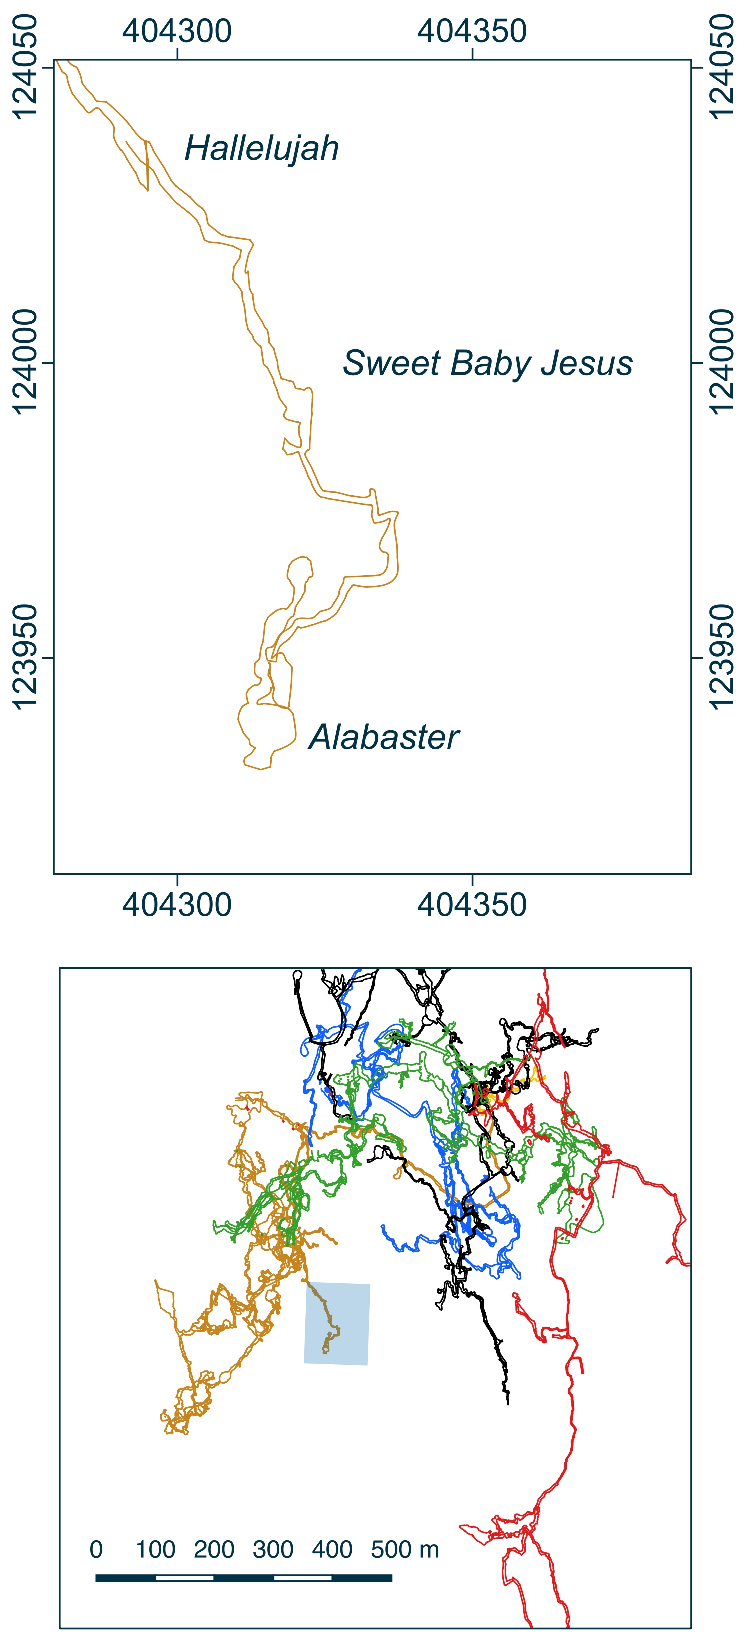
\includegraphics[width=\linewidth]{images/little_insets/sbj_inset.pdf}
	\caption{Plan view of the \protect\passage{Hallelujah} branch. Slovenian National Grid ESPG 3794}
	\label{Sweet baby Jesus inset}
\end{marginfigure}

Soon enough, we started seeing little notes ‘Unexplored’ pointing in different directions off the main passage.  Again looking at the instruction sheet, we carried on into a lovely small phreatic tube, then through a sandy squeeze into the terminal chamber of '\passage{Sweet baby Jesus}', the termination of exploration. The way on, the ‘unknown’ was a simple passage leading off from that small chamber. Gathering our kit, discarding what we thought would be unnecessary from here, we stepped off along the stooping, white horizontal passage. 

I had a little apprehension concerning what would follow: it seemed every lead my hand had touched this year degenerated or ended. I’d seen a too tight muddy squeeze, a blue sump at shallow level, a flat roofed chamber filled with scree and a drippy boulder choke with no way out. But after each corner, the passage continued, at a shallow gradient, dotted with deep pools and sharp bends where it was necessary to crouch near the water level to pass through. It continued until we hit a pitch head. It was maybe 6m, no more, bending towards the left and away from \passage[cave]{Primadona}, which was a good sign. 

\begin{pagefigure} \centering
\includegraphics[width=\linewidth]{"images/2017/tanguy-alabaster-2017/three-outside-krn".jpg}
\caption{Tanguy Racine, Jack Hare and Larry Jiang contemplate the distant Krn massif --- Rhys Tyers}
\end{pagefigure}

This was quickly bolted and at the bottom we were confronted with a fault controlled passage again, which seemed to close down ahead. There was a deep trench in the floor, through which we could see another chamber of similar size. It was possible to climb down and double back underneath, which I did without great enthusiasm as I could see no way on at either end of the chamber. I cursed and went to the far side as a matter of fact to ascertain that the way on was elsewhere. \bignote{To my surprise, the far rift had a continuation at right angle to the chamber}, and from my vantage point, I saw another pitch head, ready for bolting. 

The first couple of metres were entertaining, the walls made of a white powdery rock, with rounded nodules protruding from all sorts of places. It looked for the first time as though it could grow to be a big find, as the pitch got spacious towards the bottom. The wall rocks, white or pale grey became more rugged and solid. At the base of the next drop, we looked around to gauge what kind of passage might lead off. We were now in a rift of respectable dimensions, the way down wide open at a larger pitch, perhaps 20m, split two-thirds of the way down by a large ledge. William also scurried off upstream of the passage to an aven (ten metres), the floor of which was a circular room with deep mud banks on either side. Where small pebbles had landed on the mud, they had shielded it from the winnowing action of the water and now stood a centimetre above the mud. All of them looked like an army of little lead soldiers, each with a distinctly coloured hat. 



We set about rigging the larger drop, putting a Y-hang above a little parallel shaft which rejoined the main pitch at the ledge. Carefully feeding as much rope as I could through the knots, we managed to reach the ledge, but just. Then, out of rope, we looked at the continuing pitch. Unfortunately, there were only a few stones on the clean, white ledge and we only had a couple of attempts each at judging how far down the next pitch went. 

There certainly was a storming continuation to the passage, and \bignote{looking at the survey, it is still headed towards blank space}, with the rest of \passage[cave]{Primadona} around 150m to the west. This had been made possible by the perseverance of the previous teams who hadn’t turned back at the first hurdle or declared the passage ‘terminated, too tight, dead’ and gone back day after day to lengthen the branch.  Thanks to their effort, Will and I had  a really good trip and left the lead better than we found it. We called it \passage{Alabaster}, after the pristine, creamy white colour of the walls.

Out of rope. Admittedly we hadn’t taken a huge amount (around 50m), but it was still a little frustrating to be short of finishing the pitch, especially since it was unlikely to be revisited this year.  With that in mind we pulled up the last rope, the other pitches being bone dry were left rigged, and surveyed back to '\passage{Sweet Baby Jesus}'. When we  finally tied in our survey to the PSS, it was getting late and since we had to cave the next day to start the derig, decided against further pushing. 

Back on the surface, when asked by Tetley what had happened, the description came in bullet points as exhaustion and hunger prevented me from stringing words into a sentence. We were soon presented with mess tins full of hot tasty food, and as the tiredness ebbed away we entered the survey data into the surface computer. The realisation that \bignote{we were still going and had lost around 40m of elevation}, with more depth to come completed the feeling of elation after what had been, for me personally, a reward after so many harder exploration trips.

\name{Tanguy Racine}
